\documentclass{article}
\usepackage{amsmath}
\usepackage[hidelinks]{hyperref}
\usepackage{pythonhighlight}
\usepackage{pgfplots}
\pgfplotsset{compat = newest}
\setlength\parindent{0pt}

\begin{document}
    \hyperlink{activation_functions}{\textbf{Activation functions}}
    \begin{itemize}
        \item \hyperlink{relu}{Relu}
        \item \hyperlink{sigmoid}{Sigmoid}
        \item \hyperlink{softmax}{Softmax}
        \item \hyperlink{tanh}{Tanh}
    \end{itemize}

    \hyperlink{layers}{\textbf{Layers}} \\
    \hyperlink{losses}{\textbf{Loss functions}} \\
    \hyperlink{models}{\textbf{Models}} \\
    \clearpage

    \hypertarget{activation_functions}{\textbf{Activation functions}} \\

    Activation functions are mathematical functions applied to
    the output of a neuron in neural network. They introduce non-linearity into 
    the model so it can learn more complex patterns. \\

    An Activation class is Layer subclass that can be attached to a \hyperlink{layers}{\underline{layer}} 
    (another Layer subclass) in the network. \\

    Activation class:
    \begin{python}
class Activation(Layer):
    def __init__(self, activation_function) -> None:
        activation = activation_functions.get_function(activation_function)
        self.name = activation_function
        self.activation = activation[0]
        self.activation_derivative = activation[1]

    def forward(self, input_data):
        self.input = input_data
        self.output = self.activation(self.input)
        return self.output

    def backward(self, output_error):
        return self.activation_derivative(self.input, output_error)
    \end{python}
    \pagebreak

    \hypertarget{relu}{\underline{ReLU function}} \\
    
    ReLU (Rectified Linear Unit) is an activation function that returns 0 for all 
    negative input values and the input value itself for all 
    positive values. \\

    \begin{align*}
        f(x) = max(0, x)
    \end{align*}
    \begin{center}
    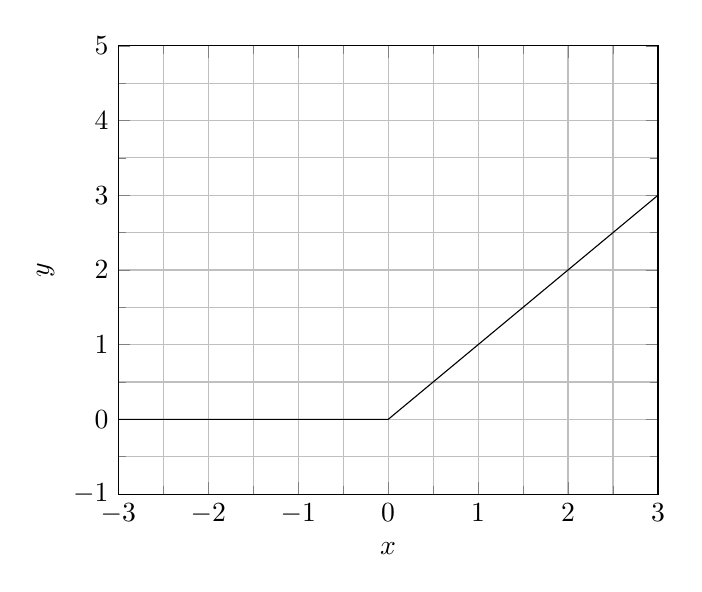
\begin{tikzpicture}
        \begin{axis}[
            xmin=-3, xmax=3,
            ymin=-1, ymax=5,
            xtick distance = 1.0,
            ytick distance = 1.0,
            grid = both,
            minor tick num = 1,
            major grid style = {lightgray},
            xlabel = {$x$},
            ylabel = {$y$},
        ]
            \addplot[] {max(0,x)};
        \end{axis}
    \end{tikzpicture}
    \end{center}
    \pagebreak

    \hypertarget{sigmoid}{\underline{Sigmoid function}} \\

    Sigmoid is an activation function that maps input values 
    to a range between 0 and 1. \\

    \begin{align*}
        f(x) = \frac{1}{1 + e^{-x}}
    \end{align*}

    \begin{center}    
    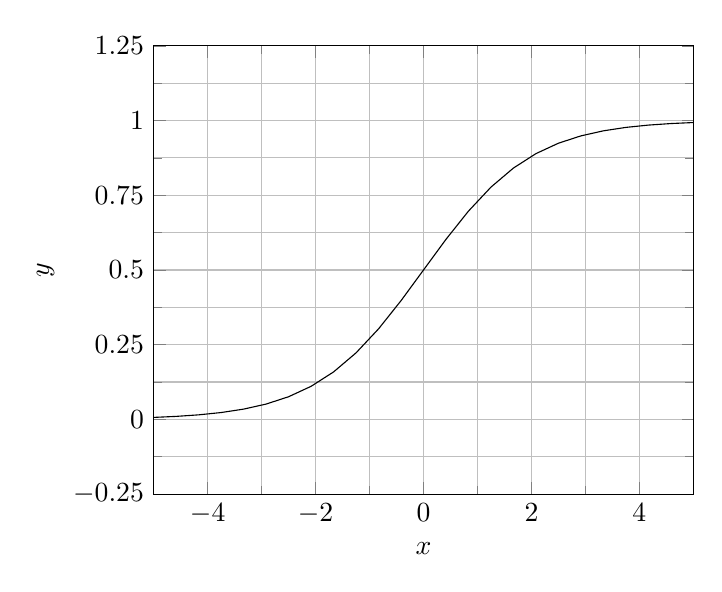
\begin{tikzpicture}
        \begin{axis}[
            xmin=-5, xmax=5,
            ymin=-0.25, ymax=1.25,
            xtick distance = 2.0,
            ytick distance = 0.25,
            grid = both,
            minor tick num = 1,
            major grid style = {lightgray},
            xlabel = {$x$},
            ylabel = {$y$},
        ]
            \addplot[] {1/(1+exp(-x))};
        \end{axis}
    \end{tikzpicture}
    \end{center}
    \pagebreak

    \hypertarget{softmax}{\underline{Softmax function}} \\

    Softmax is an activation function used for multi-class classification
    problems. It takes a vector of raw scores (logits) and converts 
    them into a probability distribution over multiple classes meaning that 
    each value will be in range $[0, 1]$ and the sum of those values is 1.
    \begin{align*}
        y(x_{i}) = \frac{e^{x_{i}}}{\sum_{j=1}^{N} e^{x_{j}}}
    \end{align*}
    
    NB! Because the derivative for Softmax function is calculated 
    together with Categorical Cross Entropy loss, they can only be 
    used in combination with each other. The last layer of the model
    should have Softmax as the activation function and the model should 
    use Categorical Cross Entropy loss. \\
    \pagebreak

    \hypertarget{tanh}{\underline{Tanh function}} \\

    Tanh is an activation function that maps input values to a range 
    between -1 and 1.
    \begin{align*}
        f(x) = \frac{e^{x} - e^{-x}}{e^{x} + e^{-x}}
    \end{align*}

    \begin{center}    
        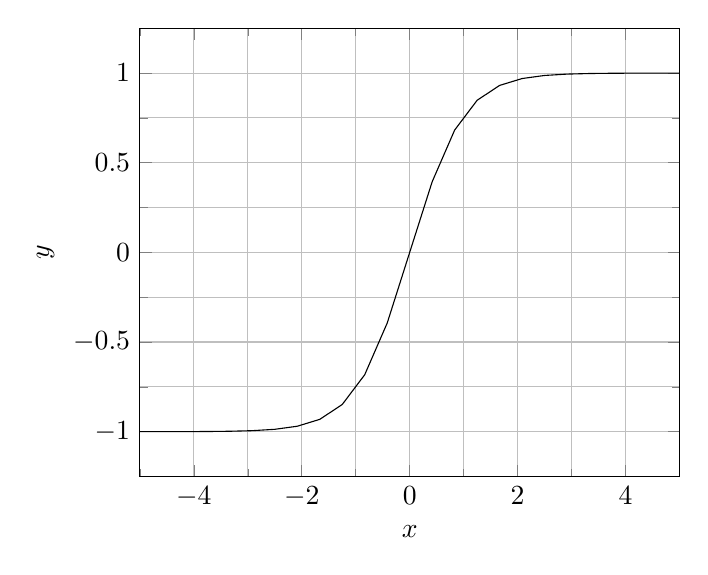
\begin{tikzpicture}
            \begin{axis}[
                xmin=-5, xmax=5,
                ymin=-1.25, ymax=1.25,
                xtick distance = 2.0,
                ytick distance = 0.5,
                grid = both,
                minor tick num = 1,
                major grid style = {lightgray},
                xlabel = {$x$},
                ylabel = {$y$},
            ]
                \addplot[] {(exp(x)-exp(-x))/(exp(x)+exp(-x))};
            \end{axis}
        \end{tikzpicture}
        \end{center}
    \clearpage

    \hypertarget{layers}{\textbf{Layers}} \\

    Layer is a functional unit that takes input data, applies a 
    mathematical transformation to it and produces an output. Each layer 
    consists of a set of neurons each of which computes a weighted sum of 
    its inputs and applies an activation function to the result. \\

    Base layer class:
    \begin{python}
class Layer:
    def __init__(self) -> None:
        self.input = None
        self.output = None

    def forward(self, input):
        raise NotImplementedError

    def backward(self, output_error, learning_rate):
        raise NotImplementedError

    def update(self, learning_rate):
        raise NotImplementedError
    \end{python}
    Each layer has a forward() function, backward() function and update() function. Forward function
    calculates the output given an input, backward function calculates the gradients that will be applied to 
    the weights and update function updates the weights accordingly.
    \clearpage

    \hypertarget{losses}{\textbf{Loss functions}}
    \clearpage

    \hypertarget{models}{\textbf{Models}}
    \clearpage
\end{document}